
\documentclass[10pt,openany,a4paper]{article}
\usepackage{tikz, pgfplots, tkz-euclide,calc}
\usetikzlibrary{patterns,shapes.arrows,calc}
\usepackage{fancyhdr}
\usepackage{enumerate,enumitem}
\usepackage{cancel}
\usepackage{varwidth}

% TAMBAHKAN PACKAGE SENDIRI KALAU KURANG

\usepackage{geometry}
\geometry{
	left = 22mm,
	right = 22mm,
	top = 25mm,
	bottom = 25mm,
}
\usepackage{graphicx}
\usepackage{subcaption}
\usepackage{soul}
\usepackage{hyperref}
\usepackage{float}
\usepackage{setspace}
\usepackage{afterpage}
\usepackage{xcolor}
\usepackage[nosectionbib]{apacite}
\usepackage{lmodern}
\usepackage{mathtools}
\usepackage{upgreek}
\usepackage{siunitx}
% \usepackage{fontawesome5}
\usepackage{fontawesome6}
\usepackage{physics}
\usepackage{pdfpages}
\usepackage{hyperref}
\renewcommand{\baselinestretch}{1.3}
\usepackage{multicol}
\usepackage{hyperref,ragged2e,amsmath,multicol,gensymb,setspace,
fancyhdr,amsfonts,tikz,pgfplots,nccmath,enumerate,verbatim,amsthm,physics}
\usepgfplotslibrary{polar,fillbetween}
% Disable tikz externalization to avoid requiring -shell-escape
\usepgfplotslibrary{external}
\tikzexternalize[prefix=tikz/]
\tikzset{reuse path/.code={\pgfsyssoftpath@setcurrentpath{#1}}}
\usetikzlibrary{shapes.geometric,arrows}
\newcommand\mylog[1]{\mathop{{}^{#1}\mathrm{log}}}
\pgfplotsset{compat=1.15}
\pgfplotsset{my style/.append style={axis x line=middle, axis y line=
middle, xlabel={$x$}, ylabel={$y$}, axis equal }}
\usepackage{etoolbox}
% remove stray \makeatother
\newtheorem{defn}{Definisi}[section]
\newtheorem{teo}[defn]{Teorema}
\newtheorem{thm}{Teorema}[section]
\newtheorem{lemma}{Lemma}
\newtheorem{lemmas}[defn]{Lemma}
\newtheorem{cor}[defn]{Akibat}
\newtheorem{asumsi}[defn]{Asumsi}
\theoremstyle{definition}
\newtheorem{con}{Contoh}[section]
\theoremstyle{definition}
\theoremstyle{plain}
\newtheorem{prop}{Proposisi}[section]
\renewcommand{\proofname}{Bukti}
\renewcommand{\thethm}{\arabic{chapter}.\arabic{thm}}

\newcommand{\normlp}[1]{\left\|#1\right\|_{L^p_{\lambda}(0,T;H)}}% Fungsi norm (||x||)
\newcommand{\R}{\mathbb{R}}
\renewcommand{\natural}{\mathbb{N}}
\newcommand{\Xpl}{X^R_{p,\lambda}}
\newcommand{\Xpls}{X^R_{p,\lambda^*}}
\newcommand{\qpl}{q^R_{p,\lambda}}
\newcommand{\qpls}{q^R_{p,\lambda^*}}
\pagestyle{fancy}
\fancyhf{}
\lhead{Halaman \thepage}
\cfoot{\faXTwitter\ \href{https://x.com/ahmadzakiyudin_/}{@ahmadzakiyudin\_} | \faInstagram\ \href{https://instagram.com/ahmadzakiyudin_/}{@ahmadzakiyudin\_} | \faTiktok\ \href{https://tiktok.com/@ahmathz/}{@ahmathz}}
\rhead{Soal ETS \\ Kalkulus 1 ITS 2025/2026}
\hypersetup{
    colorlinks=true,
    linkcolor=blue,
    filecolor=blue,      
    urlcolor=blue,
}
\newenvironment{jawab}[2][tes]{
% \fbox{\begin{minipage}{14.65cm}
\textbf{Kata kunci materi:} #1.\\
\textbf{Penyelesaian:} #2
% \end{minipage}}
}{}

\newenvironment{jawab2}[2][tes]{
\fbox{\begin{minipage}{14.65cm}
 #2
\end{minipage}}}{}

\newenvironment{jawaban}[2][tes]{
\colorlet{oldcolor}{.}
        \color{red}
        \setlength{\fboxrule}{1pt}\boxed{\color{oldcolor}#2}\color{oldcolor}.
}{}

\newenvironment{jawaban2}[2][tes]{
\colorlet{oldcolor}{.}
        \color{red}
        \setlength{\fboxrule}{1pt}\fbox{\color{oldcolor}#2}\color{oldcolor}.
}{}

\newenvironment{penting}[2][tes]{
\colorlet{oldcolor}{.}
\color{blue}
\fbox{\color{oldcolor}#2}\color{oldcolor}
}{}

\begin{document}
% \begin{titlepage}
%     \vspace*{\fill}
%     \begin{center}
%       \Huge {PEMBAHASAN SOAL EAS \\ KALKULUS II \\ TAHUN 2024/2025}\\[0.4 cm]
%       \huge {Ahmad Hisbu Zakiyudin}\\[0.2 cm]
%       \Large {(\href{https://instagram.com/ahmadzakiyudin_/}{@ahmadzakiyudin\_})}
%     \end{center}
%     \vspace*{\fill}
%   \end{titlepage}
% !TEX root = ../../BookTemplate.tex
%%%%%%%%%%%%%%%%%%%%%%%%%%%%%%%%%%%%%%%%%%%%%%%%%%%%%%%%%%%%%%%%%%%%%%%%%%%%%%%%%%
% \begin{titlepage}
%     \raggedleft	
% 	\hspace{.025\textwidth}
% 	\parbox[b]{\textwidth}{
%     \vspace{1.5cm}
% 		{\Huge\bfseries Pembahasan Soal EAS}                \\[20pt]
% 		{\huge\textit\ Kalkulus II}\\ \\[10pt]
%         {\Large\textsc{Tahun 2024/2025}}}
% \vfill
% \rule{1pt}{.14\textheight}
% \hspace{.025\textwidth}
%     \raisebox{10pt}{\parbox[b]{.95\textwidth}{ 
%         {\Large\textsc{Ahmad Hisbu Zakiyudin}}              \\[10pt]
%         \large{\href{https://instagram.com/ahmadzakiyudin_/}{@ahmadzakiyudin\_}}               \\[25pt]
%         {\large 5 Juni 2026}}}
% \end{titlepage}
\begin{titlepage}
	\centering % Center everything on the title page
	% \scshape % Use small caps for all text on the title page
	\vspace*{1.5\baselineskip} % White space at the top of the page
% ===================
%	Title Section 	
% ===================

	\rule{13cm}{1.6pt}\vspace*{-\baselineskip}\vspace*{2pt} % Thick horizontal rule
	\rule{13cm}{0.4pt} % Thin horizontal rule
	
		\vspace{0.75\baselineskip} % Whitespace above the title
% ========== Title ===============	
	{	\Huge Soal ETS\\ 
			\vspace{4mm}
		Kalkulus 1 \\ \vspace{2mm} \huge{Tahun 2025/2026}\\	}
% ======================================
		\vspace{0.75\baselineskip} % Whitespace below the title
	\rule{13cm}{0.4pt}\vspace*{-\baselineskip}\vspace{3.2pt} % Thin horizontal rule
	\rule{13cm}{1.6pt} % Thick horizontal rule
	
		\vspace{1.75\baselineskip} % Whitespace after the title block
% =================
%	Information	
% =================
{\large Diketik ulang oleh: Ahmad Hisbu Zakiyudin}
	% {\large Oleh: Ahmad Hisbu Zakiyudin \\
	% 	\vspace*{1.2\baselineskip}
	% \href{https://instagram.com/ahmadzakiyudin_/}{@ahmadzakiyudin\_}} \\
	\vfill
	\vspace{1mm}
\huge{Selamat Belajar!}
\end{titlepage}
\makeatletter
\setlength\fboxsep{3pt}
% ensure enough header height for fancyhdr
\setlength{\headheight}{24pt}
 \begin{center}
	{\underline{\textbf{\MakeUppercase{Soal ETS Kalkulus 1 Tahun 2025/2026}}}}
    \end{center}

    \begin{center}
	\begin{tabular}{lcl}
		Mata kuliah/SKS & : & Kalkulus 1 ( SM234101 ) / 3 SKS\\
		Hari, Tanggal & : & Senin, 13 Oktober 2025\\
		Waktu & : & 07.00 - 08.40 / 100 menit\\
		Sifat & : & Tertutup\\
		Kelas & : & 40-49, 62-66\\
  ~
	\end{tabular}
    
    \noindent\rule{\textwidth}{2.pt}
        \end{center}
    \begin{enumerate}
     \item Dapatkan semua nilai \(x\) yang memenuhi pertidaksamaan
    \[
        \dfrac{2x + 1}{3x - 6} < \dfrac{1}{2}.
    \]

    \item Diberikan fungsi \(f(x) = \frac{1}{x-1}\) dan \(g(x) = 2 - \sqrt{x}\).
    \begin{enumerate}
        \item Tentukan domain dari fungsi \(f\) dan \(g\).
        \item Dapatkan fungsi \((f \circ g)(x)\) beserta domainnya.
    \end{enumerate}

    \item Diberikan fungsi \(f(x) = \begin{cases} \frac{x^3-8}{2x-4}, & x \neq 2 \\ k, & x=2 \end{cases}\).
    \begin{enumerate}
        \item Tentukan nilai \(k\) sehingga \(f(x)\) kontinu di \(x = 2\).
        \item Berdasarkan hasil dari (a), nyatakan \(f(x)\) sebagai polinomial.
    \end{enumerate}

    \item Diberikan fungsi implisit \(3x^2 + y^2 - 2xy + y - x = 6\). Tentukan \(\frac{dy}{dx}\) di titik \((0,-3)\).

    \item Diketahui garis \(g_1: y = -x + 6\) dan garis \(g_2: y = 2x\).
    \begin{enumerate}
        \item Tentukan titik potong kedua garis \(g_1\) dan \(g_2\).
        \item Tentukan titik potong \(g_1\) dengan garis \(x = 1\).
        \item Tentukan pula titik potong \(g_2\) dengan garis \(x = 1\). Gambarkan sketsa ketiga garis \(g_1\), \(g_2\), dan garis \(x = 1\). Hitung luas segitiga yang dibentuk ketiga garis tersebut.
    \end{enumerate}
\end{enumerate}
\newpage
 \begin{center}
	{\underline{\textbf{\MakeUppercase{Soal ETS Kalkulus 1 Tahun 2025/2026}}}}
    \end{center}

    \begin{center}
	\begin{tabular}{lcl}
		Course / Credit & : & Kalkulus 1 ( SM234101 ) / 3 SKS\\
		Day, Date & : & Monday, 13 October 2025\\
		Time / Exam Time & : & 09.00 - 10.40 / 100 menit\\
		Type & : & Tertutup\\
		Class & : & 1, 4, 67, 70, 71\\
  ~
	\end{tabular}
    
    \noindent\rule{\textwidth}{2.pt}
        \end{center}
\begin{enumerate}
           \item Solve the following inequality.
    \[ \frac{x^2 - x - 12}{x^2 - 2x - 3} \ge 0. \]

    \item Given a function \(f(x) = 2 - \sqrt{x}\) and \(g(x) = \frac{1}{x-1}\). Determine:
    \begin{enumerate}
        \item[a)] The domain of function \(f\) and \(g\);
        \item[b)] Function \((f \circ g)(x)\) and its domain.
    \end{enumerate}

    \item Write the derivative formula of \(\frac{f}{g}\), that is \(\frac{d}{dx}\left(\frac{f(x)}{g(x)}\right)\). \\
    Then, find the derivative of \(\frac{f}{g}\) given that \(f(x) = 2x^2 + 3x - 2\) and \(g(x) = x - 1\) for \(x \neq 1\).

    \item Given \(f(x) = \begin{cases} \frac{x^3-8}{2x-4}, & x \neq 2 \\ 2k, & x=2 \end{cases}\).
    \begin{enumerate}
        \item[a.] Determine k such that \(f(x)\) continuous at \(x = 2\).
        \item[b.] Based on the result of a), rewrite \(f(x)\) as a polynomial.
    \end{enumerate}

    \item Sketch the base curve \(x = y^2\). Based on that base curve, use translation to sketch the curve \(x = y^2 + 4y + 1\). (Explain the process).

        \end{enumerate}
               \newpage
 \begin{center}
	{\underline{\textbf{\MakeUppercase{Soal ETS Kalkulus 1 Tahun 2025/2026}}}}
    \end{center}

    \begin{center}
	\begin{tabular}{lcl}
		Mata kuliah/SKS & : & Kalkulus 1 ( SM234101 ) / 3 SKS\\
		Hari, Tanggal & : & Senin, 13 Oktober 2025\\
		Waktu & : & 11.00 - 12.40 / 100 menit\\
		Sifat & : & Tertutup\\
		Kelas & : & 17-22\\
  ~
	\end{tabular}
    
    \noindent\rule{\textwidth}{2.pt}
        \end{center}
\begin{enumerate}
    \item \begin{enumerate}
        \item Nyatakan pernyataan $\sqrt{(2x-1)^2}$ dalam bentuk nilai mutlak.
        \item Dapatkan semua nilai $x$ yang memenuhi persamaan $\sqrt{(2x-1)^2}=1-2x$.
    \end{enumerate}
    \item Diberikan fungsi $f(x)=\sqrt{x-4}$.
    \begin{enumerate}
        \item Tentukan domain dan range dari fungsi $f(x)$.
        \item Tentukan $f^{-1}(x)$, domain dan range dari $f^{-1}(x)$.
    \end{enumerate}
    \item Diberikan persamaan separuh lingkaran 
    \begin{align*}
       x=4+\sqrt{-y^2+14y-24}.
    \end{align*}
    \begin{enumerate}
        \item Dapatkan pusat dan jari-jari lingkaran. 
        \item Sketsa grafiknya.
    \end{enumerate}
    \item Diketahui fungsi $f(x)=\left(\frac{3}{x}+x^2\right)^{3/2}$. Dapatkan $f'(2)$.
    \item Diberikan $f(x)=\begin{cases}
        \frac{\sqrt{x+9}-3}{x}, &x\neq 0\\
        \frac{1}{3}k-\frac{1}{5}, &x=0,
    \end{cases}, \text{dengan } x\in [-9,\infty)$.\\
    Tentukan nilai $k$ sehingga $\displaystyle\lim_{x\to 0}f(x)=f(0)$.\\
    Kemudian nyatakan fungsi $f(x)$ tanpa menggunakan bentuk fungsi sepotong-sepotong dalam domainnya untuk nilai $k$ yang diperoleh.
\end{enumerate}
\newpage
 \begin{center}
	{\underline{\textbf{\MakeUppercase{Soal ETS Kalkulus 1 Tahun 2025/2026}}}}
    \end{center}

    \begin{center}
	\begin{tabular}{lcl}
		Mata kuliah/SKS & : & Kalkulus 1 ( SM234101 ) / 3 SKS\\
		Hari, Tanggal & : & Senin, 13 Oktober 2025\\
		Jam/Waktu Ujian & : & 13.30 - 15.10 / 100 menit\\
		Sifat & : & Tertutup\\
		Kelas & : & 13-16, 50-61\\
  ~
	\end{tabular}
    
    \noindent\rule{\textwidth}{2.pt}
        \end{center}
        \begin{enumerate}
            \item \begin{enumerate}
                \item Definisikan $|3-x|$.
                \item Berdasarkan point (a) tersebut, tentukan semua nilai $x$ yang memenuhi pertidaksamaan 
                \begin{align*}
                    |3-x|\leq -2x+1.
                \end{align*}
            \end{enumerate}
            \item \begin{enumerate}
                \item Tentukan jarak titik $(1,3)$ dan $(7,11)$.
            \item Tentukan persamaan lingkaran yang diameternya adalah jarak titik $(1,3)$ ke $(7,11)$. 
            \end{enumerate}
            \item Diberikan fungsi $f(x)=\begin{cases}
                x-1, &x<3\\
                2(x-4)^2, &x\geq 3
            \end{cases}$.
            \begin{enumerate}
                \item Dapatkan $f(3)$, $f(-2)$, dan $f(1-x^2)$.
                \item Dapatkan domain dan range dari $f(x)$.
                \item Sketsa grafik dari $f(x)$.
            \end{enumerate}
            \item Diberikan $f(x)=\frac{x^3-1}{x-1}$.
            \begin{enumerate}
                \item Tentukan $\displaystyle\lim_{x\to 1}f(x)$.
                \item Buatlah sketsa grafik $y=f(x)$.
            \end{enumerate}
            \item Diketahui kurva $x^2y+4x-3y^2=2$.
            \begin{enumerate}
                \item Dapatkan $\frac{dy}{dx}$ dengan menggunakan turunan fungsi implisit.
                \item Dari (a) dapatkan persamaan garis singgung pada kurva tersebut di titik $(1,1)$.
            \end{enumerate}
        \end{enumerate}
\newpage
 \begin{center}
	{\underline{\textbf{\MakeUppercase{Soal ETS Kalkulus 1 Tahun 2025/2026}}}}
    \end{center}

    \begin{center}
	\begin{tabular}{lcl}
		Mata kuliah/SKS & : & Kalkulus 1 ( SM234101 ) / 3 SKS\\
		Hari, Tanggal & : & Selasa, 14 Oktober 2025\\
		Waktu & : & 07.00 - 08.40 / 100 menit\\
		Sifat & : & Tertutup\\
		Kelas & : & 113 dan 114\\
  ~
	\end{tabular}
    
    \noindent\rule{\textwidth}{2.pt}
        \end{center}
        \begin{enumerate}
            \item Dapatkan penyelesaian dari pertidaksamaan 
            \begin{align*}
                \frac{x^2-x-12}{x^2+3x-10}\geq 0.
            \end{align*}
            \item \begin{enumerate}
                \item Dapatkan kemiringan garis $\ell$ yang melalui titik $(0,0)$ dan $(-2,1)$.
                \item Jika garis $\ell$ tegak lurus dengan garis yang menyinggung lingkaran yang berpusat di $(0,0)$ dan berjari-jari $\sqrt{5}$, di titik $(-2,1)$, maka dapatkan persamaan garis singgung lingkaran tersebut dan sketsalah.
            \end{enumerate}
            \item Tuliskan rumus turunan dari $fg$ yaitu $\frac{d}{dx}(f(x)g(x))$\\
            Selanjutnya, dapatkan turunan dari $fg$, jika diketahui $f(x)=3x^2-7x$ dan $g(x)=3-2x^2$.
            \item Dapatkan $\displaystyle \lim_{x\to 3} \frac{\sqrt{3x+7}-4}{x-3}$.
            \item Diberikan fungsi $f(x)=\frac{1}{x-1}$ dan $g(x)=x^2$.
            \begin{enumerate}
                \item Dapatkan $(f\circ g)(x)$.
                \item Jika diketahui $(p\circ g)(x)=  x^2-3$, dapatkan $p(x)$.
            \end{enumerate}
        \end{enumerate}

\newpage
 \begin{center}
	{\underline{\textbf{\MakeUppercase{Soal ETS Kalkulus 1 Tahun 2025/2026}}}}
    \end{center}

    \begin{center}
	\begin{tabular}{lcl}
		Course / Credit & : & Kalkulus 1 ( SM234101 ) / 3 SKS\\
		Day, Date & : & Tuesday, 14 October 2025\\
		Time / Exam Time & : & 07.00 - 08.40 / 100 menit\\
		Type & : & Closed\\
		Class & : & 2, 3, 68, 69\\
  ~
	\end{tabular}
    
    \noindent\rule{\textwidth}{2.pt}
        \end{center}
        \begin{enumerate}
            \item Find the solution of the following inequality 
            \begin{align*}
                \frac{x^2-x-12}{x^2+3x-10}\geq 0.
            \end{align*}
            \item \begin{enumerate}
                \item Find the gradient of the line $\ell$ which goes through $(0,0)$ and $(-2,1)$.
                \item If line $\ell$ is perpendicular with the line that tangent with a circle centered at $(0,0)$ and radius $\sqrt{5}$, at $(-2,1)$, then find the aforementioned tangent line equation and sketch the graph. 
            \end{enumerate}
            \item Write the derivative formula of $fg$ that is $\frac{d}{dx}(f(x)g(x))$\\
            Then, find the derivative of $fg$, given that $f(x)=3x^2-7x$ and $g(x)=3-2x^2$.
            \item Calculate $\displaystyle \lim_{x\to 3} \frac{\sqrt{3x+7}-4}{x-3}$.
            \item Given a function $f(x)=\frac{1}{x-1}$ and $g(x)=x^2$. 
            \begin{enumerate}
                \item Find $(f\circ g)(x)$.
                \item Given $(p\circ g)(x)=  x^2-3$, then find $p(x)$.
            \end{enumerate}
        \end{enumerate}
               \newpage
 \begin{center}
	{\underline{\textbf{\MakeUppercase{Soal ETS Kalkulus 1 Tahun 2025/2026}}}}
    \end{center}

    \begin{center}
	\begin{tabular}{lcl}
		Mata kuliah/SKS & : & Kalkulus 1 ( SM234101 ) / 3 SKS\\
		Hari, Tanggal & : & Selasa, 14 Oktober 2025\\
		Waktu & : & 09.00 - 10.40 / 100 menit\\
		Sifat & : & Tertutup\\
		Kelas & : & 5-12, 23-29, 115 dan 116\\
  ~
	\end{tabular}
    
    \noindent\rule{\textwidth}{2.pt}
        \end{center}
        \begin{enumerate}
            \item Selesaikan pertidaksamaan berikut 
            \begin{align*}
                \frac{1}{x+2} \leq \frac{2}{x-1}.
            \end{align*}
            \item Gambarkan kurva dasar $y=\frac{1}{x}$. Berdasarkan kurva dasar tersebut, gunakan translasi (pergeseran) untuk menggambar kurva $y=\frac{1}{x-2}+4$ (Jelaskan ilustrasinya).
            \item Diberikan fungsi $f(x)=\frac{1}{x-2}$ dan $g(x)=\sqrt{5-x}$. Tentukan :
            \begin{enumerate}
                \item Domain fungsi $f$ dan $g$.
                \item Fungsi $(f\circ g)(x)$ dan $\left(\frac{f}{g}\right) (x)$ beserta domainnya masing-masing. 
            \end{enumerate}
            \item Tunjukkan bahwa $f(x)=\begin{cases}
                3x+1, &x\leq 2\\
                x+5, &x>2
            \end{cases}$ adalah fungsi kontinu tetapi tidak dapat diturunkan di $x=2$.
            \item Tentukan $\dfrac{dy}{dx}$ jika $x^2y+y^3=10$.
        \end{enumerate}
               \newpage
 \begin{center}
	{\underline{\textbf{\MakeUppercase{Soal ETS Kalkulus 1 Tahun 2025/2026}}}}
    \end{center}

    \begin{center}
	\begin{tabular}{lcl}
		Mata kuliah/SKS & : & Kalkulus 1 ( SM234101 ) / 3 SKS\\
		Hari, Tanggal & : & Selasa, 14 Oktober 2025\\
		Waktu & : & 11.00 - 12.40 / 100 menit\\
		Sifat & : & Tertutup\\
		Kelas & : & 102, 108-112\\
  ~
	\end{tabular}
    
    \noindent\rule{\textwidth}{2.pt}
        \end{center}
        \begin{enumerate}
            \item Dapatkan solusi dari ketaksamaan 
            \begin{align*}
                2<|3-x|\leq 5.
            \end{align*}
            Petunjuk: Gunakan rumus jarak.
            \item Diketahui garis $\ell_1$ dengan gradien $m_1=\frac{2}{3}$ dan garis $\ell_2$ berpotongan tegak lurus dengan $\ell_1$ di titik $(4,-1)$. Dapatkan persamaan garis $\ell_2$. \\
            Gambarkan kedua garis $\ell_1$ dan $\ell_2$ pada satu bidang koordinat. 
            \item Diketahui $f(x)=x^2-4x$.
            \begin{enumerate}
                \item Tentukan domain alami untuk $x$ agar $f(x)$ mempunyai invers.
                \item Dapatkan $f^{-1}(x)$, domain, dan rangenya. 
            \end{enumerate}
            \item Diberikan fungsi 
            \begin{align*}
                f(x)=\begin{cases}
                    \frac{x^2-9}{x+3}, &x\neq -3\\
                    k, &x=-3
                \end{cases}
            \end{align*}
            \begin{enumerate}
                \item Tentukan nilai $k$ agar $f(-3)=\displaystyle\lim_{x\to -3} f(x)$.
                \item Dengan memberi $k$ pada $\displaystyle\lim_{x\to-3} f(x)$, tunjukkan bahwa $f(x)$ dapat dinyatakan sebagai fungsi polinomial. 
            \end{enumerate}
            \item Diketahui $f(x)=(\sqrt{x}+2x^2+1)^5$.\\
            Dengan aturan rantai, dapatkan turunan pertama dari $f(x)$.
        \end{enumerate}
               \newpage
 \begin{center}
	{\underline{\textbf{\MakeUppercase{Soal ETS Kalkulus 1 Tahun 2025/2026}}}}
    \end{center}

    \begin{center}
	\begin{tabular}{lcl}
		Mata kuliah/SKS & : & Kalkulus 1 ( SM234101 ) / 3 SKS\\
		Hari, Tanggal & : & Selasa, 14 Oktober 2025\\
		Waktu & : & 15.30 - 17.10 / 100 menit\\
		Sifat & : & Tertutup\\
		Kelas & : & 30-39\\
  ~
	\end{tabular}
    
    \noindent\rule{\textwidth}{2.pt}
        \end{center}
        \begin{enumerate}
            \item Dapatkan penyelesaian dari pertidaksamaan 
            \begin{align*}
                2\leq x^2-2\leq 7.
            \end{align*}
            \item Gunakan grafik dasar $x=y^2$ dan sifat pergeseran/translasi untuk menggambar parabola $x=y^2+2y+3$.
            \item Tentukan domain dari fungsi $(f\circ g)(x)$ jika diketahui fungsi $g(x)=2x+3$ dengan $0\leq x<3$ dan fungsi $f$ terdefinisi pada interval $-1\leq x <5$.
            \item Diberikan fungsi $f(x)=\left|\dfrac{x^2-9}{x-3}\right|$. Dapatkan titik $x$ di mana membuat fungsi $f(x)$ diskontinu?\\
            Dapatkan nilai fungsi $f(x)$ pada titik tersebut agar menjadi kontinu dan sketsa grafik fungsi tersebut.
            \item Dengan diferensiasi implisit, dapatkan $\frac{dy}{dx}$ dari $x^3y^2-3xy^2+x=1$.
        \end{enumerate}
 \newpage
 \begin{center}
	{\underline{\textbf{\MakeUppercase{Soal ETS Matematika Tahun 2025/2026}}}}
    \end{center}

    \begin{center}
	\begin{tabular}{lcl}
		Mata kuliah/SKS & : & Matematika ( SM234152 ) / 2 SKS\\
		Hari, Tanggal & : & Jumat, 17 Oktober 2025\\
		Waktu & : & 07.00 - 08.40 / 100 menit\\
		Sifat & : & Tertutup\\
		Kelas & : & 1-8\
  ~
	\end{tabular}
    
    \noindent\rule{\textwidth}{2.pt}
        \end{center}
\begin{enumerate}
    \item Diberikan SPL 
    \begin{align*}
        x+y+2z &= 8\\
        -x-2y+3z &= 1\\
        3x-7y+4z &= 10
    \end{align*}
    \begin{enumerate}
        \item Nyatakan SPL tersebut dalam bentuk persamaan matriks $A\mathbf{x}=b$.
        \item Menggunakan Eliminasi Gauss, carilah solusi (jika ada) dari SPL tersebut.
    \end{enumerate}
    \item Carilah himpunan penyelesaian dari pertidaksamaan
    \begin{align*}
        1<|3x-4|\leq 6.
    \end{align*}
    \item Tentukan nilai $k$ agar garis $\ell_1:kx-3y=12$ tegak lurus dengan garis $\ell_2:2x+3y=6$.
    \item Selesaikan persamaan berikut 
    \begin{align*}
        \ln \left(\frac{1}{x}\right)+\ln(4x^3)=2.
    \end{align*}
    \item Diberikan sistem persamaan fungsi permintaan dan penawaran (\textit{supply and demand})
    \begin{align*}
       4P=-Q_d+93\\
       5P=Q_s+33
    \end{align*}
    dengan $P,Q_d,Q_s$ masing-masing adalah harga, jumlah permintaan (\textit{demand}), dan jumlah penawaran (\textit{supply}).
    \begin{enumerate}
        \item Jika harga barang $Rp5.000$, berapa jumlah unit permintaan>
        \item Jika jumlah barang yang ditawarkan 17 unit, berapa harga penawarannya.
        \item Tentukan harga dan jumlah barang di titik equilibrium.
        \item Gambarkan/sket kurva penawaran dan permintaan dan titik keseimbangannya.
    \end{enumerate}
\end{enumerate}
\newpage 

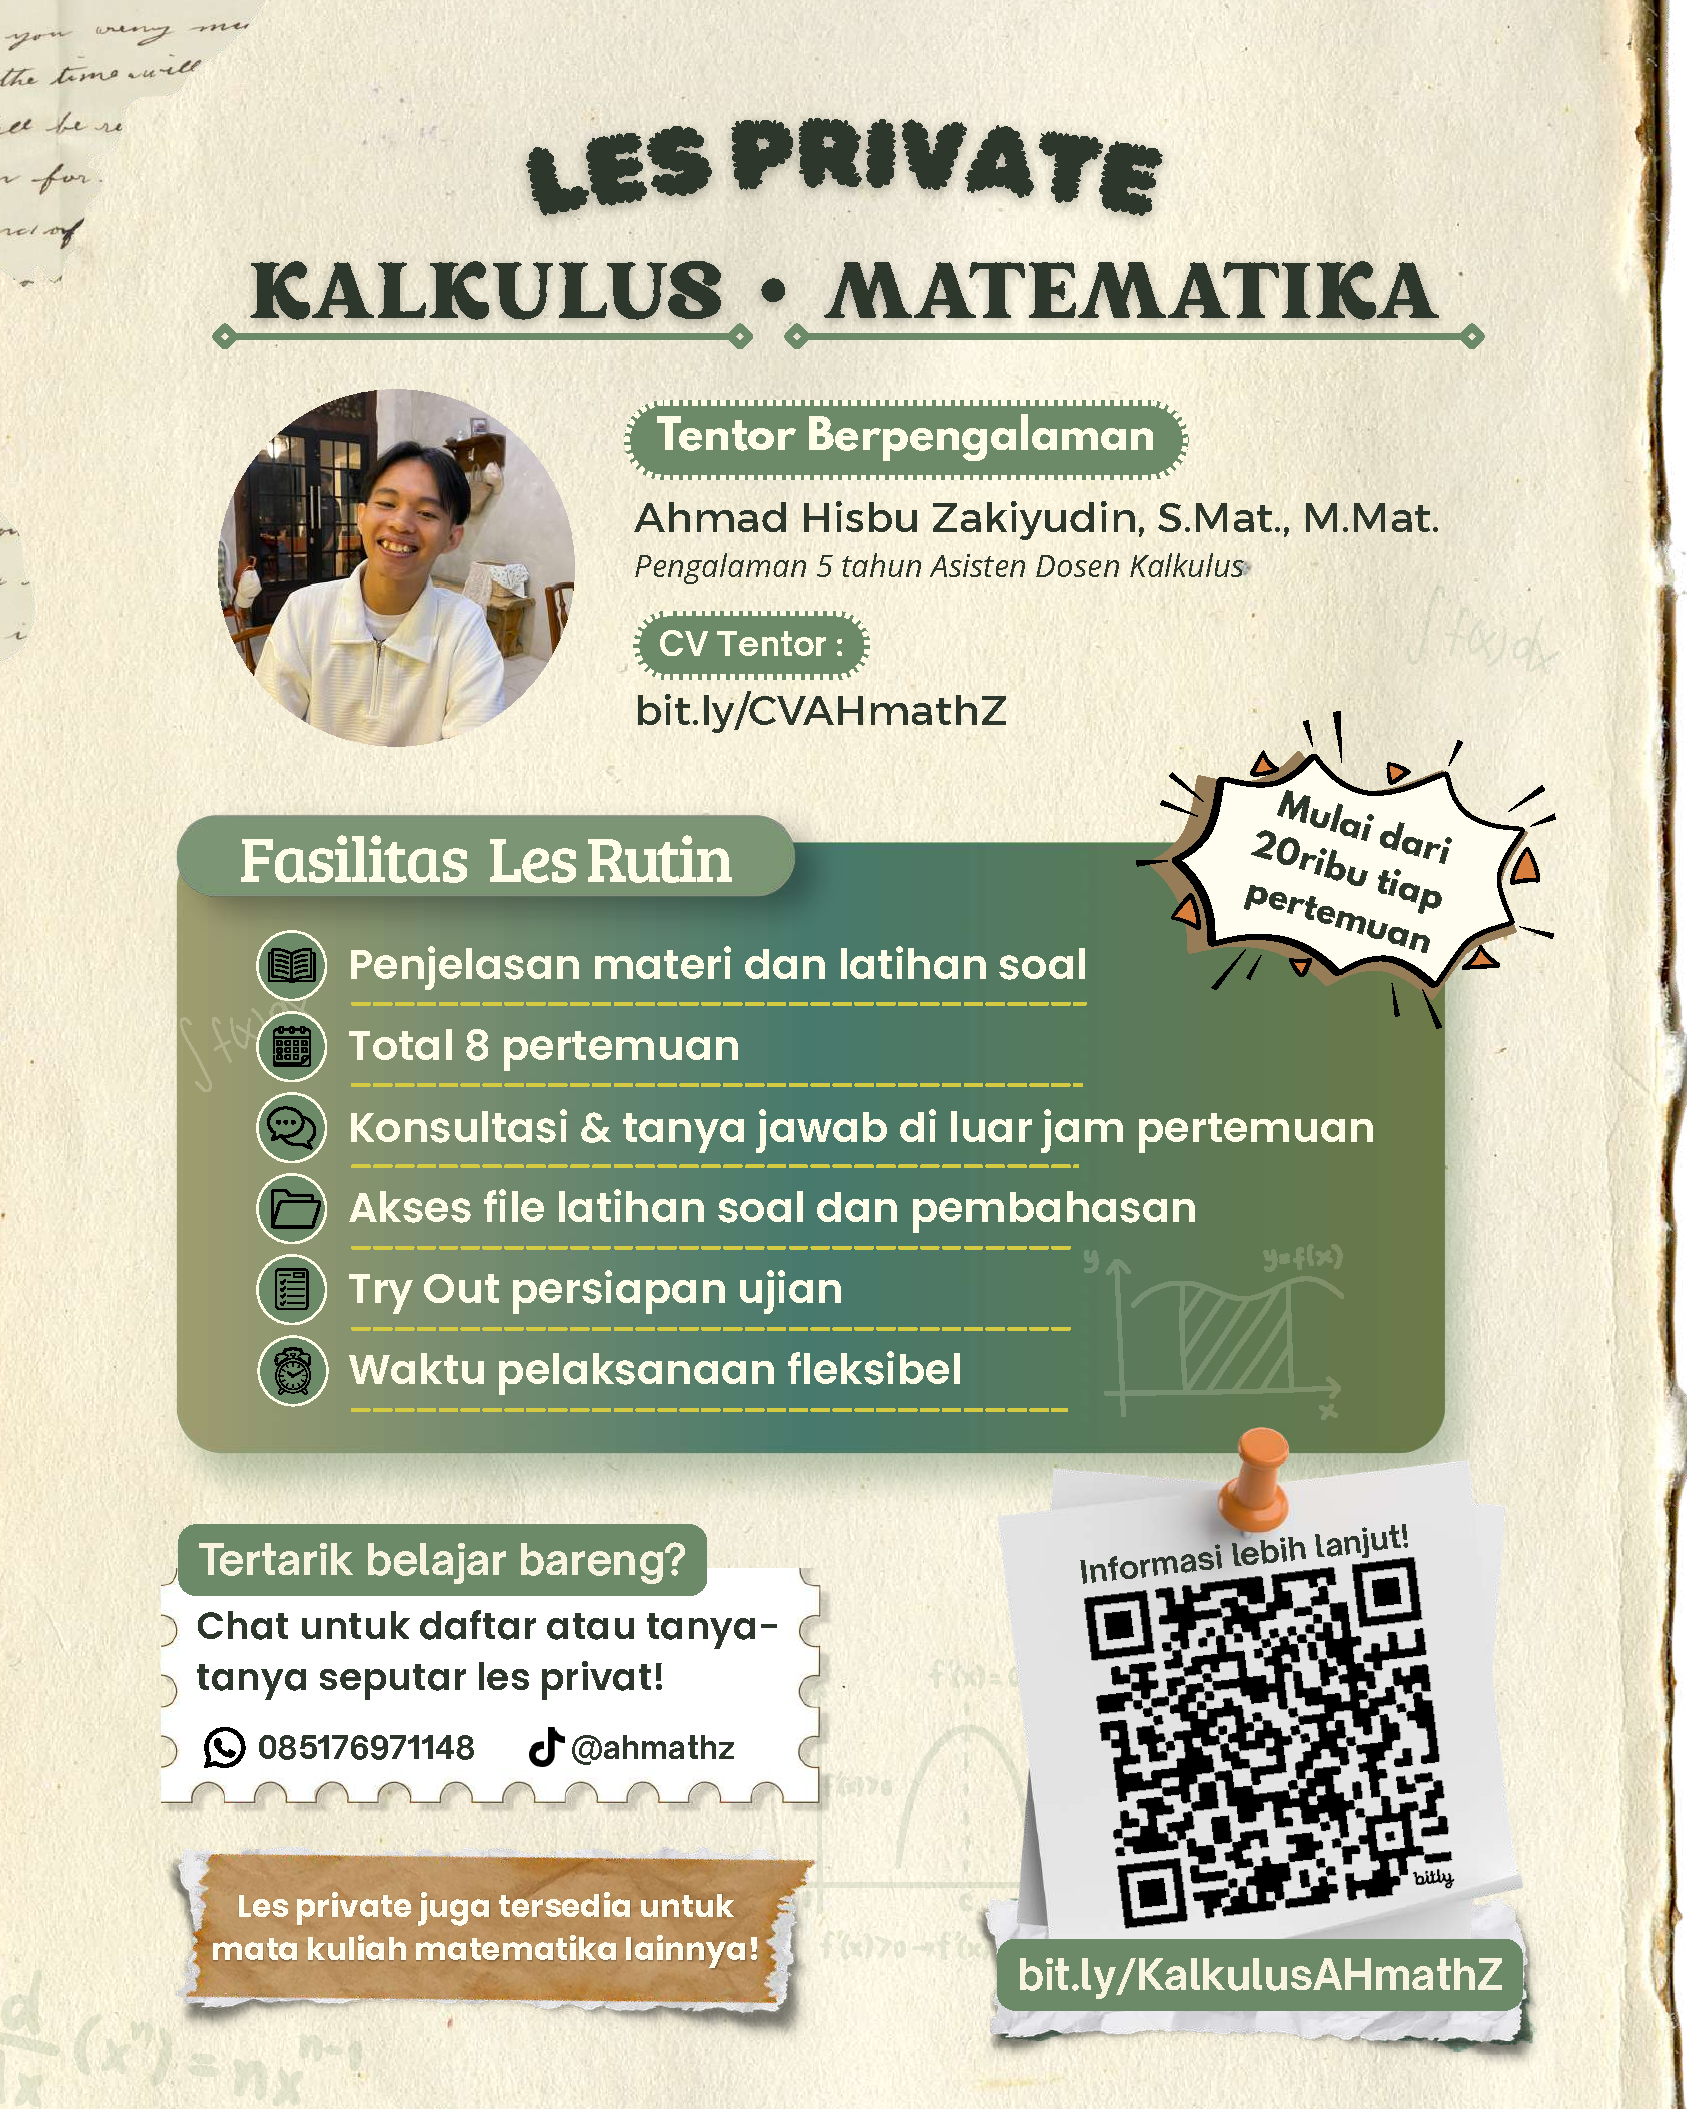
\includepdf[pages=-]{les.pdf}

\end{document}


